\documentclass[tikz, border=1mm]{standalone}

%% FEYNMAN DIAGRAMS
\usepackage[compat=1.1.0]{tikz-feynman}
\tikzfeynmanset{warn luatex=false}

\begin{document}
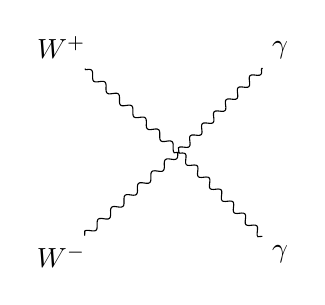
\begin{tikzpicture}
  \begin{feynman}
    \vertex (a);
    \vertex [above left=of a](i1) {\(W^{+}\)};
    \vertex [below left=of a] (i2) {\(W^{-}\)};
    \vertex [above right=of a] (f1) {\(\gamma\)};
    \vertex [below right=of a] (f2) {\(\gamma\)};

    \diagram* {
      (i1) -- [boson] (a) -- [boson] (i2),
      (f1) -- [boson] (a) -- [boson] (f2),
    };
  \end{feynman}
\end{tikzpicture}
\end{document}
